\chapter{基于深度相机的静态模型的采集}

 本文通过捕捉物体形变获取形变关键帧,然后根据关键帧相对于静态模型的相对形变构建形变子空间,
 这些工作都需要获取物体的静态模型作为参照。
 本章的目的就是借助深度相机,获取一个物体静态三维模型,作为后续形变捕捉与形变子空间构建的输入。
\begin{figure}[h]
    \centering
    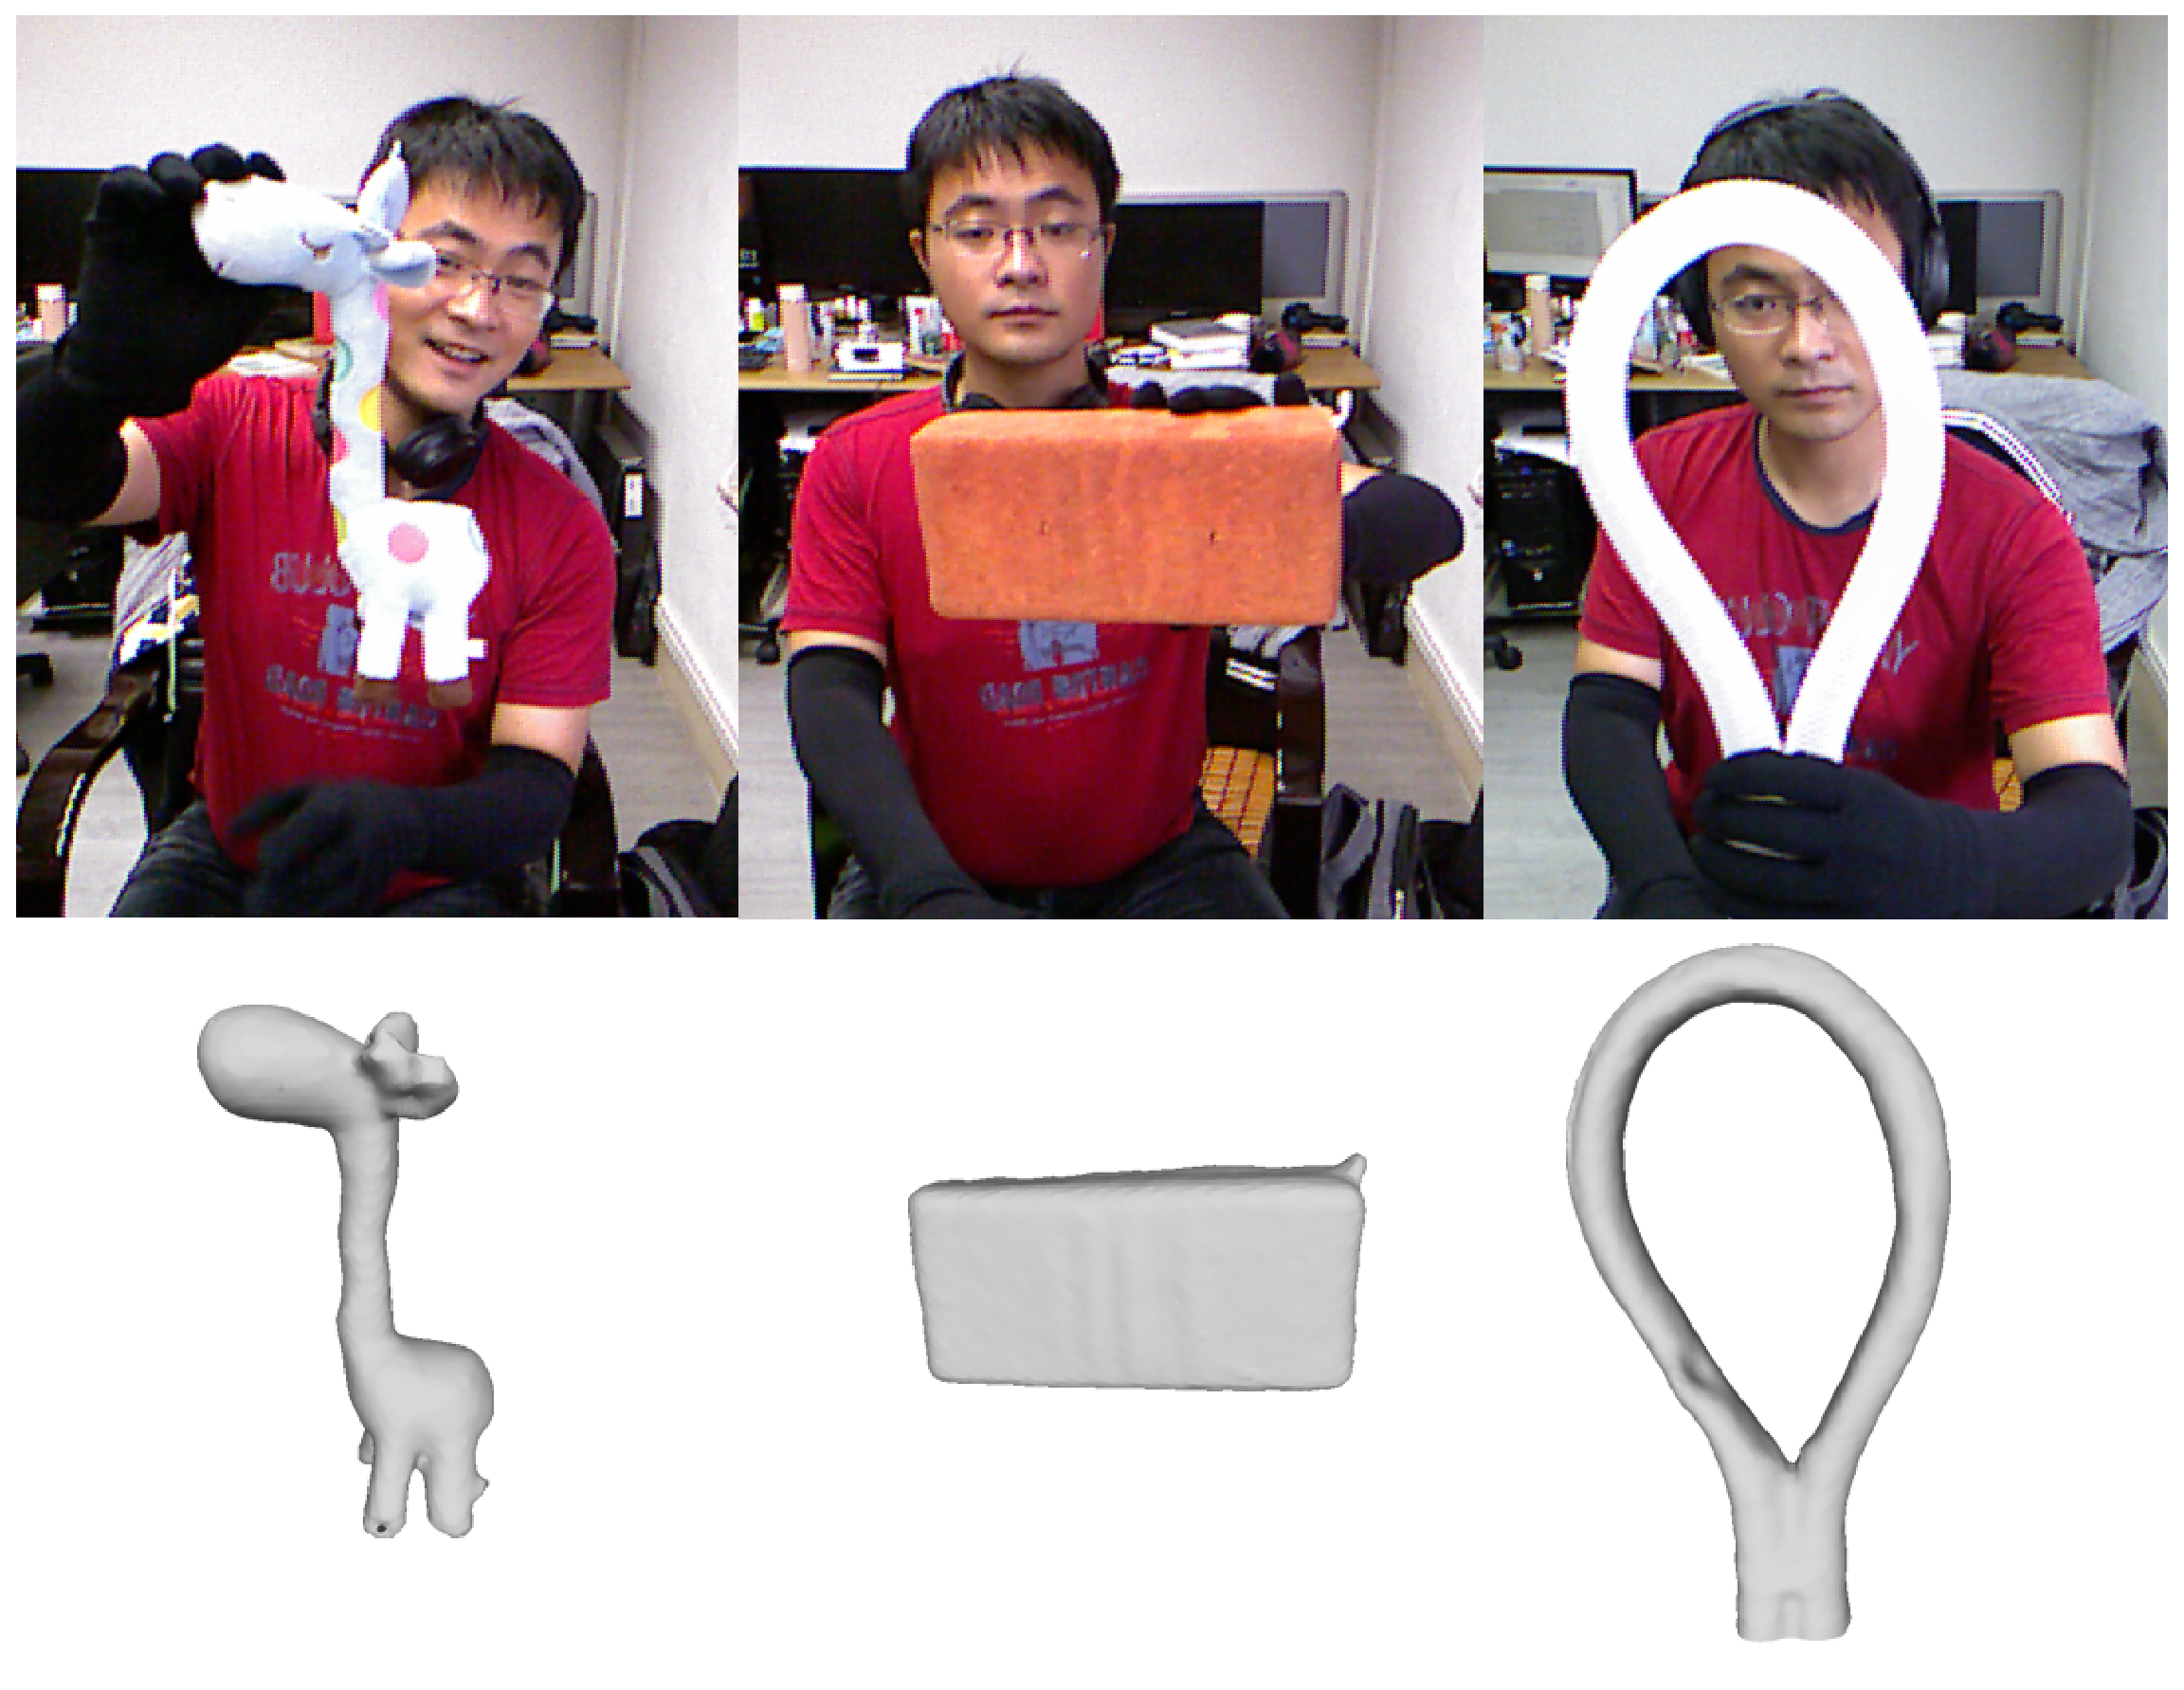
\includegraphics[width=0.9\textwidth]{./Pictures/static_mesh.eps}
    \caption{采集静态模型}
    \label{static_model}
\end{figure}

\section{基于深度相机的三维重建概述}
对于现实世界中存在的物体,其三维模型通常可以通过CAD软件建模或者借助扫描设备重建。
本文所使用的模型均借助深度相机重建。
\begin{figure}[h]
    \centering
    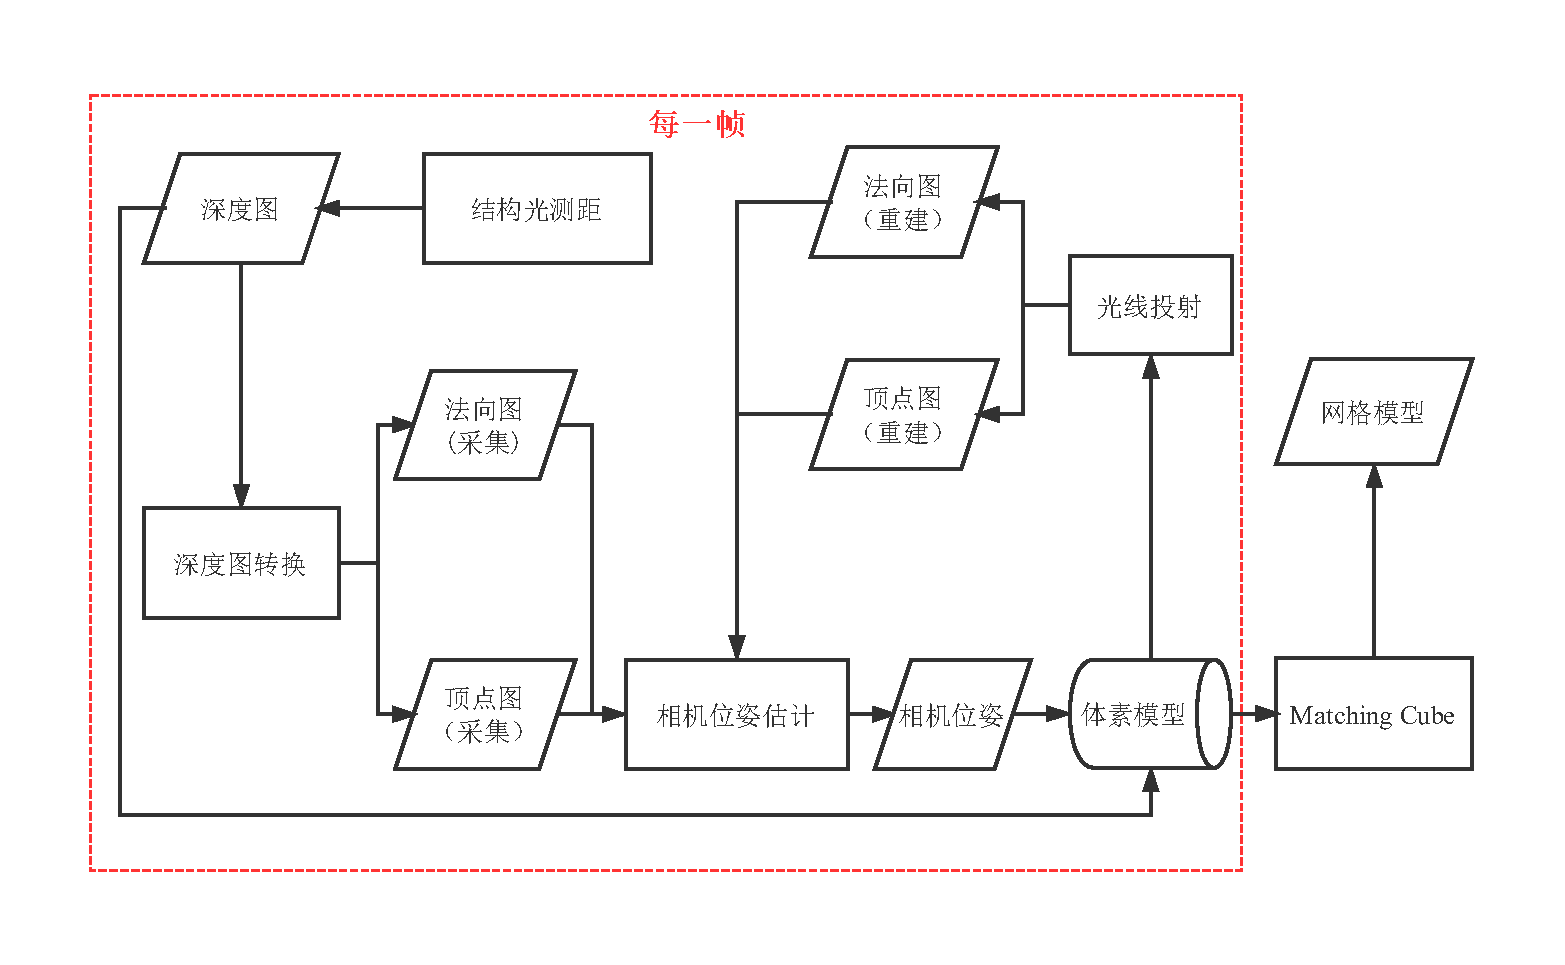
\includegraphics[width = 0.9\textwidth]{./Pictures/kf_pipeline_cropped.pdf}
    \caption{三维重建流程}
    \label{kfpipeline}
\end{figure}

深度相机是一种可以获取深度信息的设备,即能够测量物体表面距离相机的距离。
如同章节\ref{range_finding}所说,现在较为流行的三维测距技术有飞行时间、三角测距和结构光。
本文采用的是Microsoft生成的Kinect一代,这是一台基于结构光技术的深度相机。
Kinect除了能够获得RGB图像外,还能获得深度图像。
深度图像的每个像素记录的是物体表面距离相机的距离,
利用透视原理,可以推算出物体表面和相机的相对位置。
三维重建算法就可以通过扫描过程中获取的深度信息重建出物体的几何信息,获得三维模型。

\section{三维重建流程}
本文采用的是KinectFusion算法\cite{izadi2011kinectfusion},
能够实时的借助深度相机重建三维模型。
KinectFusion算法\cite{izadi2011kinectfusion}以深度视频(由深度图像组成的图像流)为输入。
对于每一帧,会计算场景中物体和相机的相对位置(物体在相机坐标系中的位置),
得到当前相机采集的顶点位置信息和法向信息。
同时算法还会计算,相机在世界坐标系(通常是第一帧的相机坐标)中的位置,
并将每一帧获得的数据融合到一个统一的体素模型中,从而得到物体的三维模型。
如图\ref{kfpipeline}所示,对于每一帧输入,算法可主要分为深度图转换、相机位姿估计、
体素模型融合和光线投射四个步骤。

\subsection{深度图转换}
深度相机获取的数据是深度图像,每个像素记录的是每个采样点到相机的距离。
由于在相机位姿估计阶段,我们需要通过计算相邻两帧点云发生的刚体变换,
我们需要将深度图转换为点云数据。
点云数据记录的每个顶点的位置和法向,分别存储在顶点图和法向图中。
深度图转换就是要将原始的深度图转换为顶点图和法向图。

时刻$i$获取的深度图$\bm{D_i}$中的一个像素$\bm{u}=(x,y)$
对应着三维空间中的一个顶点$\bm{v_i}(\bm{u})$。
根据相机成像原理,可得到以下公式:
\begin{equation}
    \bm{v_i(u)}=\bm{D_i}(u)\bm{K}^-1[\bm{u},1]
\end{equation}
其中$K$是Kinect深度相机的内参矩阵。
对于深度图像中的每一个像素,其计算是相互独立的,所以这个过程可以借助GPU并行完成,
得到顶点图$\bm{V_i}$。
在得到顶点图后,顶点的法向量就可以借助相邻顶点的信息计算得到:
\begin{equation}
    \bm{n_i}(\bm{u})=(\bm{v_i}(x+1,y)-\bm{v_i}(x,y))\times(\bm{v_i}(x,y+1)-\bm{v_i}(x,y))
\end{equation}
其中$\bm{v_i}(x,y)$为像素点$\bm{u}(x,y)$对应的顶点坐标。
和顶点图$\bm{V_i}$一样,法向图$N_i$也可以借助GPU并行的计算。

\subsection{相机位姿估计}
深度图转换阶段得到的点云的坐标都是在相机坐标系下的,记录的是场景中物体和相机的相对位置。
由于在扫描采集的时候,相机的位置与朝向(即相机的位姿)是不断变化的。
所以为了将各帧的数据融合到一个统一的坐标系中,需要计算每一帧的6自由度(6DOF)的相机位姿。
本文采用的是ICP算法\cite{besl1992method},
是一种非常流行的用于计算三维形状对齐的算法。
该算法的核心是通过优化得到一个最优的刚体变换使得两个点云的对应点的误差最小,
关于该算法的详细内容可以查阅Besl的论文\cite{besl1992method}。
在这一步中,ICP用于估计相邻两帧的点云之间发生的刚体变换。
将每一帧累计起来,就可以得到相机在世界坐标系中的位姿。

ICP最为关键也是开销较大的一步就是确定两组点云的对应关系。
由于计算的是相邻两帧间的微小的刚体变换,
上一帧$\bm{u}$位置顶点在下一帧会投影在$\bm{u}$的附近。
所以在本算法中,将两帧中投影到同一个像素点并且空间距离小于指定阈值的顶点设为对应点。

\subsection{体素模型融合}
三维重建需要得到一个单一的完整的三维模型,而对于扫描过程中的每一帧,
所获取的点云都是在不同的相机坐标系中的。
所以为了得到一个单一的三维模型,需要需要将每一帧的数据融合到一个统一的坐标系中。
本文采用体素模型记录重建过程中的三维模型。
该体素模型由体素的三维阵列组成,每个体素记录的是TSDF(Truncated SignedDistance Functions),
是SDF(Signed Distance Functions)的一个变种。
SDF描述的该体素距离物体表面的距离,在物体表面的值为0,
物体外部为正值,内部为负值,是一种隐式曲面的描述方式。
TSDF是被裁剪过的SDF,将SDF限制在一个指定的区间,仅有效记录物体表面附近体素的值。

对于每一帧输入,这一步会计算当前图像所见物体表面相应体素的值,
并和体素中已经存储的历史值求加权平均得到更新后的TSDF。
在这一步中每个体素的值是互相独立的,可以并行的计算。
由于TSDF仅仅有效的记录表面的值,所以那些不在表面附近的体素可以进行相同的计算,
却不会得到有效的更新。

\subsection{光线投射}
在相机位姿估计的步骤中,需要计算当前帧点云和上一帧点云的相对刚体变换。
其中上一帧的点云并不是相机采集的点云,
而是根据已重建的模型以及上一帧的相机位置生成的点云。
这个点云是通过光线投射(Raycast)算法得到的。

在这一步中,每一个像素点$\bm{u}$,会发射一条射线,沿着投影的反方向
(从焦点经过成像平面上的像素点射向物体)穿过射线上的体素。
在穿过体素的过程中如果TSDF的值发生了由正值到负值的符号翻转,则说明射线穿透了物体的表面,
从外部进入了内部,发生翻转的位置就是表面所在的位置,由此可以计算出该位置坐标与法向。
各像素的光线投射可以互相独立的并行的计算,从而得到顶点图和法向图。

\subsection{生成网格模型}
在三维重建的过程中本文采用体素模型

